\paragraph{Guiroma}

\subparagraph{Outline}

Treat it like vanilla SR with 4 picks per player. Small map -> early contact -> max Income T1/T2 or T3. RMO -> you can get bailed out with a dice-roll \& you also sometimes can't convert an advantage due to luck.

\url{https://www.youtube.com/watch?v=jTnh64g0Edo}
\\
\url{https://www.warzone.com/Forum/382353-allgemeine-rangordnung-der-boni-auf-guiroma}
\\
4x5, neutrals 2/4, wastelands 15/3, base: +5

\subparagraph{Map Dynamics}

Guiroma's map (Imperium Romanum) favors specific regions/bonuses. Using Figure \ref{guiroma_winrates}:

\begin{figure}[H]
  \centering
  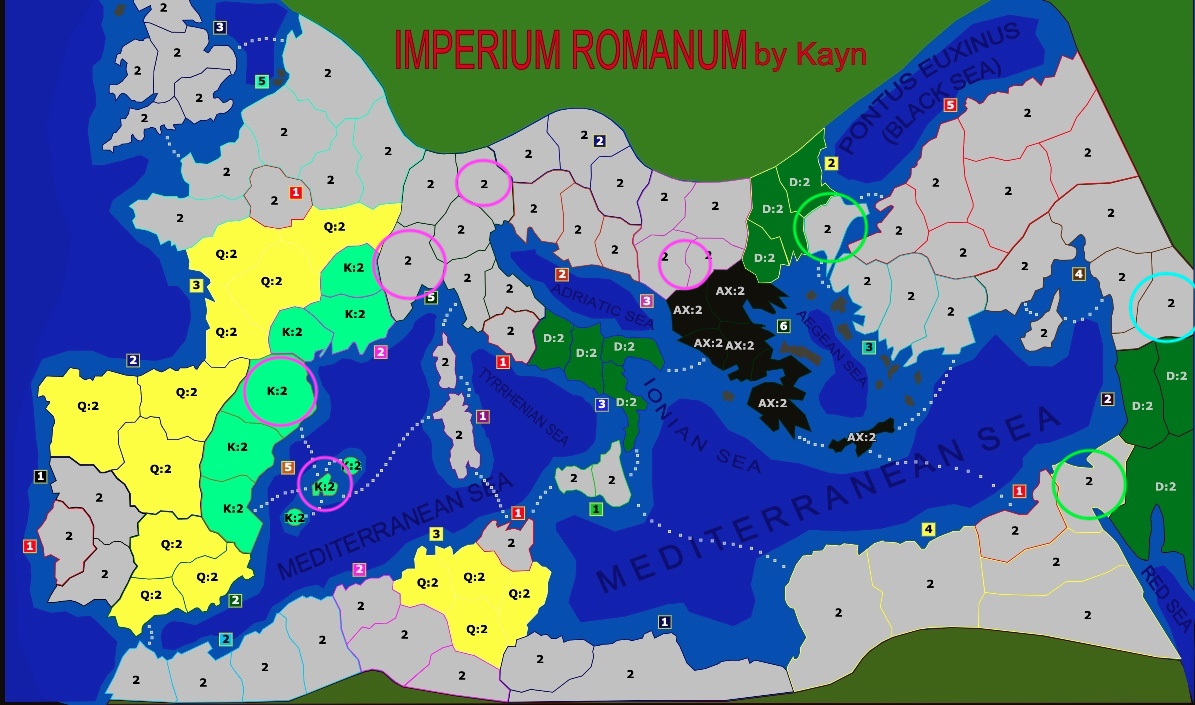
\includegraphics[width=0.9\textwidth]{Images/guiroma.jpg}
  \caption{Guiroma Chokepoints and WR}
  \label{guiroma_winrates}
\end{figure}

\begin{itemize}
    \item The map has compartments with bottlenecks that allow easy defense.
    \begin{enumerate}
        \item Asia - the whole Turkey area + Arabia. You only need to protect 3 chokepoints to control this area: Pelusium in Egypt, Crete in Greece, and Byzantium between Thracia and Asia. If you control these, you win. At the start of the game, run the algorithm:
        \begin{itemize}
            \item Can Egypt counter Arabia?
            \item Can Syria counter Arabia?
            
            If the answer to both is no, and Arabia can be picked, then Arabia is a safe but boring first pick (not always the best pick). Examples: \href{https://www.warzone.com/MultiPlayer?GameID=36627592}{1}, \href{https://www.warzone.com/MultiPlayer?GameID=36565091}{2}, \href{https://www.warzone.com/MultiPlayer?GameID=34480255}{3}. However, sometimes you might not pick Arabia first to avoid being predictable. If you lose Arabia and need coverage for Asia, the counters are basically Thracia, Greece, Sicily, and Egypt. Example: \href{https://www.warzone.com/MultiPlayer?GameID=35593018}{here}. My 5/6 are long-term Asia counters in case I lose my first pick, which of course, I lost.
        \end{itemize}    
        Asia is so good that Arabia is the most picked bonus on the map (273/450 games) with 56\% WR. Asia/Ponticia/Syria all have >50\% WR and 2/3 of it's counters, Illyricum and Thracia rock 60\% WR.
        \item The Italy/Greece region has safe and slow in expansion bonuses. In these settings of 4 spawns in such a small map, a safe spawn for max Income T1/T2 and contact is usually enough. Southern Italy +3 suffers no double border and counters Greece. This justifies it being the second-best area/bonus on the map. It's the only super-efficient bonus on the map but is counterable by almost everything. High risk, high reward.
        \item Central Europe: Usually becomes a brawl and is contested. Also might be a noob-trap.
        \item Spain/France: Tarraconensis > Southern Gaul > Narbonensis usually. All other bonuses are very situational. Great region, rich in expansion, has 2 chokepoints you'd want to secure.
        \item Central Africa: Despite appearing appealing, it has awful expansion, and usually a pick there means you don't have a cover pick in an area that outputs more income. Example: \url{https://www.warzone.com/MultiPlayer?GameID=25701044}.
    \end{enumerate}
\end{itemize}

\subparagraph{Gameplay \& Ideas}

Guiroma acts similarly to any vanilla SR template in that you want a combination of a) max Income on contact and b) better position. I have heard of an argument for RMO existing in Guiroma because in certain distributions First Pick is extremely powerful, not only due to Arabia's existence, but because in 4-pick templates 1st pick gets both first and last pick (1/4/5/8 vs 2/3/6/7). It's a controversial topic I will not delve into.
\\
\\
Max Income end of Turn 1 is 12 with a tap in a setup that has exactly 2x +2 Bonuses and a combo +3 bonus to be completed with a tap. Realistically speaking, the max Income is 11 through configurations such as:
\begin{itemize}
    \item +3 FTB, +1 like a Sicily spawn, \& a combo +2 Bonus.
    \item 2x +2 bonuses, \& a combo +2 Bonus.
\end{itemize}

In reality, the optimal transition involves a setup of 8-10 Income end of Turn 1 and 13-16 Income end of Turn 2 (as long as you plan to have contact on Turn 2 or Turn 3, which is 90\% of the time the case in Guiroma). Setups like:
\begin{itemize}
    \item \href{https://www.warzone.com/MultiPlayer?GameID=40882156}{5->9->16} with Bonuses of size 2/2/3/4. That's the max.
    \item \href{https://www.warzone.com/MultiPlayer?GameID=40882156}{5->9->15} (same game different perspective) with Bonuses of size 2/2/3/3 and a counter. Or \href{https://www.warzone.com/MultiPlayer?GameID=40742256}{5->9->15} by Octane with a 6-attack.
\end{itemize}

Illyricum rolls the map even as a double pick like \href{https://www.warzone.com/MultiPlayer?GameID=36808169}{here} and \href{https://www.warzone.com/MultiPlayer?GameID=26520244}{here} (even with a wasteland).
\\
\\
The 8th pick in Guiroma intuitively combos with the 1st pick, while the 7th combos with the 2nd. This fits games like \href{https://www.warzone.com/MultiPlayer?GameID=40568482}{this one} and the Italy synergy.
